\documentclass[12pt,a4paper,titlepage]{report}
\usepackage[utf8]{inputenc}
\usepackage[francais]{babel}
\usepackage[T1]{fontenc}
\usepackage{amsmath}
\usepackage{amsfonts}
\usepackage{amssymb}
\usepackage{graphicx}
\author{Grebic Christopher - Menin Valérian}
\title{Projet de Bases de Données}

\setlength{\topsep}{5pt}%

%%%% debut macro %%%%
\newenvironment{changemargin}[2]{\begin{list}{}{%
\setlength{\topsep}{0pt}%
\setlength{\leftmargin}{0pt}%
\setlength{\rightmargin}{0pt}%
\setlength{\listparindent}{\parindent}%
\setlength{\itemindent}{\parindent}%
\setlength{\parsep}{0pt plus 1pt}%
\addtolength{\leftmargin}{#1}%
\addtolength{\rightmargin}{#2}%
}\item }{\end{list}}
%%%% fin macro %%%%
\begin{document}
\maketitle

\section*{Description du projet}
Pour le semestre 5, nous avons dû développer une application pour informatiser la gestion d'un parc animalier.


\section*{Choix d'analyse}
Le modèle conceptuel de données choisi est assez simple. Les relations sont principalement de type 1 à N sauf pour les cas suivants :
\begin{itemize}
	\item[•] Historique d'enclos \\
	Celui-ci regroupe trois dates en tant que clé primaire. L'originalité est liée au fait que nous avons trois clés étrangères. 
	\item[•] Répartition géographique \\
	La répartition des espèces affecte une localisation géographique à une espèce.
	\item[•] Composition de régime \\
	La composition d'un régime alimentaire est définie par un aliment ainsi qu'un régime pour lesquels une quantité est alors donnée.
	\item[•] Gestion des substituts \\
	Les substituts sont simplement une clé secondaire qui fait référence à la clé primaire de la classe aliments. Cela pourrait même permettre de gérer des substituts de substituts et ainsi de suite de manière récursive.
\end{itemize}
 
~ \newline
D'une manière générale, les données sont gérées de façon à permettre la plus grande flexibilité de leur contenue. C'est-à-dire que les modifications y sont le plus facile possible.

~ \newline
A cet égard de simplicité, nous avons choisi certaines conventions concernant les types de données utilisés :
\begin{itemize}
	\item[•] Les identifiants et stocks\\
	Comme toujours les identifiants sont de type INT. \\
	Les stocks et quantités sont quant à eux de type DOUBLE car les plus petits animaux ne mangent bien évidemment pas plusieurs kilos de nourriture par jour.
	\item[•] Les noms \\
	VARCHAR d'une taille de 63 en général sauf pour des cas particuliers tels que les noms scientifiques qui sont souvent plus longs possède une taille de 127.
	\item[•] Les sexes et espèces menacées \\
	Pour les sexes, nous avions le choix entre le type TINYINT ou un ENUM. Nous avons choisi l'utilisation d'un type ENUM avec comme possibilité 'M' ou 'F'. Cela simplifie la saisie et le traitement des données. \\
	Pour En ce qui concerne le fait qu'une espèce soit menacée ou non, il était plus logique et pratique d'utiliser un TINYINT. C'est donc le choix que nous avons fait.
\end{itemize}

~ \newline
En cas de besoin d'une compatibilité de notre gestion du parc avec le système du zoo, les index suivants existent :
\begin{itemize}
	\item[•] Codes aliments
	\item[•] Localisation
	\item[•] Code enclos.
\end{itemize}

~ \newline
Nous avons définis plusieurs contraintes d'intégrités pour gérer au mieux nos données.
\begin{itemize}
	\item[•] Lorsqu'une famille est supprimée, toutes les relations entre les espèces et cette famille sont supprimées (SET NULL).
	\item[•] On empeche la suppression d'une localisation si cette localisation est utilisée par une espèce (RESTRICT)
	\item[•] Lors de la suppression d'une espèce, sa répartition et ses régimes sont supprimés (CASCADE) et ses références dans animaux sont mises à NULL (SET NULL). 
	\item[•] Lorsqu'on supprime un régime, sa composition est supprimée (CASCADE) mais on empêche la suppression d'un aliment utilisé dans un régime.
	\item[•] Quand on supprime un aliment, les aliments qui utilisent ce même aliment en tant que substitut sont mis à NULL (SET NULL).
	\item[•] Suite à la suppression d'un animal, on supprime son historique d'affiliation aux enclos.
	\item[•] Après la suppression d'un enclos,  celui-ci est supprimé de l'historique.
	\item[•] Si on supprime un soigneur, toutes les relations entre les enclos et ce soigneur sont supprimées (SET NULL).
\end{itemize}

~ \newline
Le trigger permet l'utilisation du stock substitut en cas de rupture de celui de l'aliment primaire.

\begin{figure}[h!]
	\begin{changemargin}{-3.5cm}{-4cm}
	\centering
   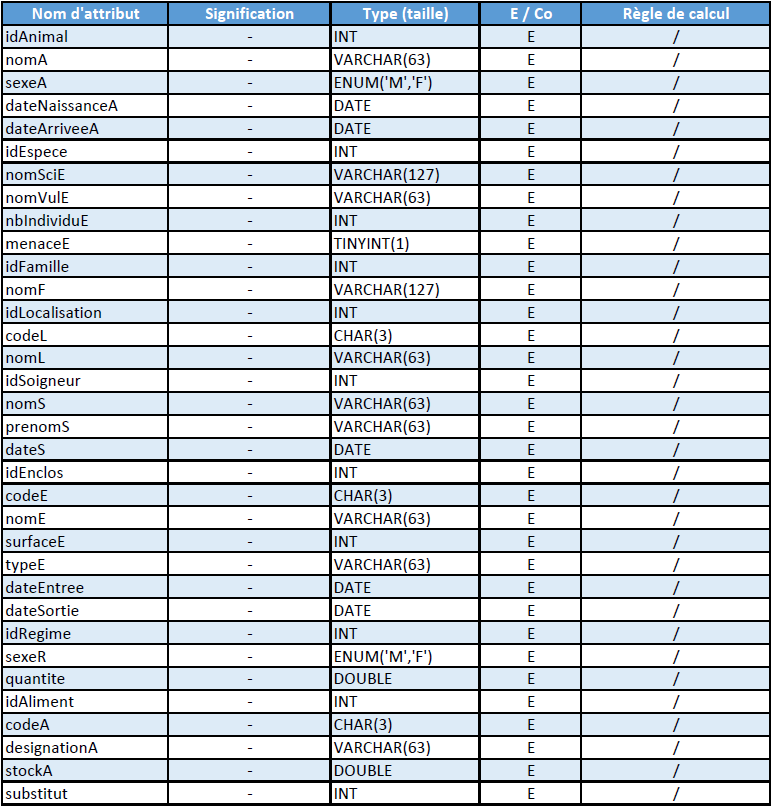
\includegraphics[scale=0.85]{dictionnaire.png}
   \caption{\label{étiquette} Dictionnaire de données}
   \end{changemargin}
\end{figure}


\begin{figure}[h!]
	\begin{changemargin}{-3.5cm}{-4cm}
	\centering
   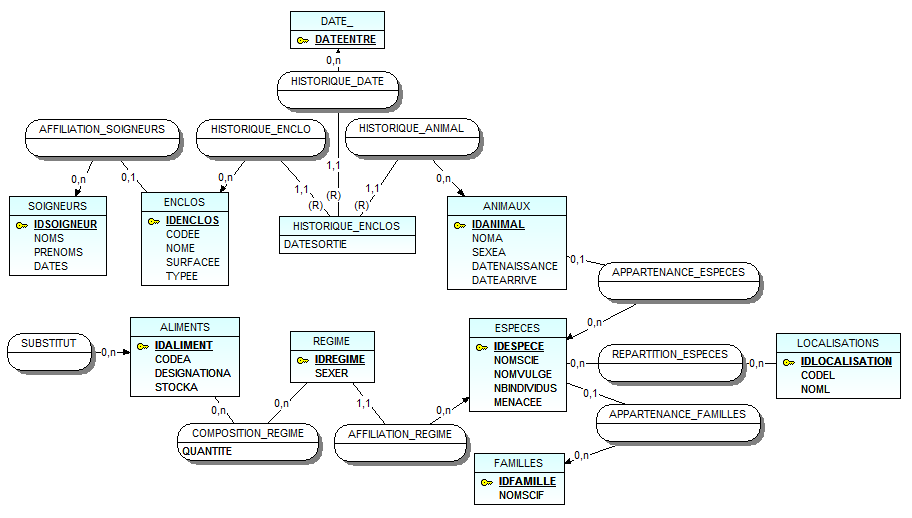
\includegraphics[angle=-90, scale=0.85]{MCD17_version3.png}
   \caption{\label{étiquette} Modèle Conceptuel de Données}
   \end{changemargin}
\end{figure}	

\begin{figure}[h!]
	\begin{changemargin}{-3.5cm}{-4cm}
	\centering
   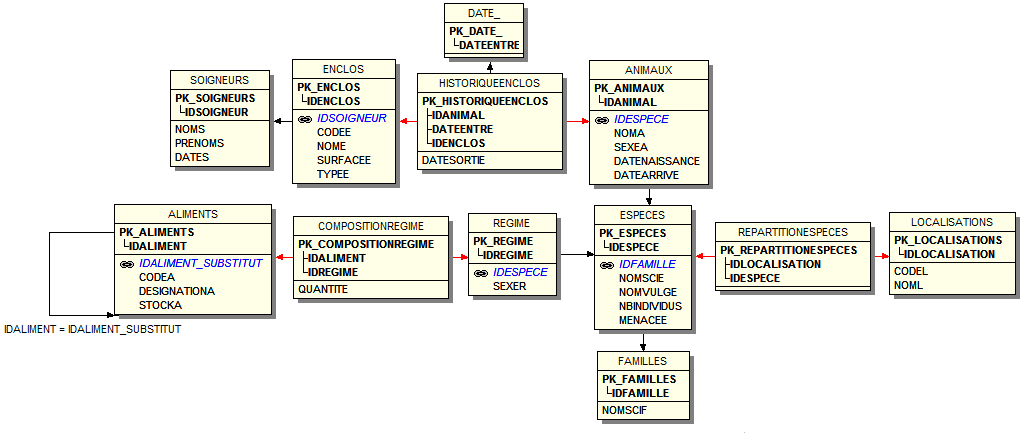
\includegraphics[angle=-90, scale=0.85]{MLR_17-12-2014version3.png}
   \caption{\label{étiquette} Modèle Conceptuel de Données}
   \end{changemargin}
\end{figure}	


\end{document}

